\documentclass[12pt]{article}
\usepackage[papersize={8cm,14cm},margin={.5cm,.5cm}]{geometry}
\usepackage{common}
\usepackage{amssymb}
\begin{document}
\begin{problem}
\item[5.] 圖(五)中,$\triangle{ABC}$ 的內切圓分別與 $\overline{BC}$、$\overline{AC}$ 相切於 $D$ 點、$E$ 點,且 $\angle B = 90^\circ$。若 $\overline{BD} = 1$,$\overline{DC} = 4$,則 $\overline{AE}$ 的長度為何?
  \begin{figure}[ht]
    \centering
    \vspace*{-1ex}
    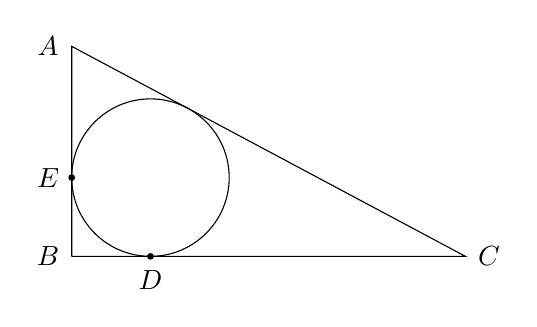
\begin{tikzpicture}
      \draw (0,0) -- (0,2.667) -- (5,0) -- (0,0);
      \draw (1,1) circle (1cm);
      \node at (-.3,2.667) {$A$};
      \node at (-.3,0) {$B$};
      \node at (5.3,0) {$C$};
      \node at (1,-.3) {$D$};
      \node at (-.3,1) {$E$};
      \filldraw (1,0) circle (1pt);
      \filldraw (0,1) circle (1pt);
    \end{tikzpicture}
    \vspace*{-1ex}
    \caption*{圖(五)}
    \vspace*{-2ex}
  \end{figure}
  \begin{choices}
    \item $\fraction{3}{2}$
    \item $\fraction{5}{2}$
    \item $\fraction{4}{3}$
    \item $\fraction{5}{3}$
  \end{choices}
\end{problem}
\end{document}
